%File: anonymous-submission-latex-2024.tex
\documentclass[letterpaper]{article} % DO NOT CHANGE THIS
\usepackage[submission]{aaai24}  % DO NOT CHANGE THIS
\usepackage{times}  % DO NOT CHANGE THIS
\usepackage{helvet}  % DO NOT CHANGE THIS
\usepackage{courier}  % DO NOT CHANGE THIS
\usepackage[hyphens]{url}  % DO NOT CHANGE THIS
\usepackage{graphicx} % DO NOT CHANGE THIS
\urlstyle{rm} % DO NOT CHANGE THIS
\def\UrlFont{\rm}  % DO NOT CHANGE THIS
\usepackage{natbib}  % DO NOT CHANGE THIS AND DO NOT ADD ANY OPTIONS TO IT
\usepackage{caption} % DO NOT CHANGE THIS AND DO NOT ADD ANY OPTIONS TO IT
\frenchspacing  % DO NOT CHANGE THIS
\setlength{\pdfpagewidth}{8.5in} % DO NOT CHANGE THIS
\setlength{\pdfpageheight}{11in} % DO NOT CHANGE THIS
%
% These are recommended to typeset algorithms but not required. See the subsubsection on algorithms. Remove them if you don't have algorithms in your paper.
\usepackage{algorithm}
\usepackage{algorithmic}
\usepackage{amsmath}
\usepackage{mathtools}
\usepackage[usestackEOL]{stackengine}
\stackMath
%
% These are are recommended to typeset listings but not required. See the subsubsection on listing. Remove this block if you don't have listings in your paper.
\usepackage{newfloat}
\usepackage{listings}
\DeclareCaptionStyle{ruled}{labelfont=normalfont,labelsep=colon,strut=off} % DO NOT CHANGE THIS
\lstset{%
	basicstyle={\footnotesize\ttfamily},% footnotesize acceptable for monospace
	numbers=left,numberstyle=\footnotesize,xleftmargin=2em,% show line numbers, remove this entire line if you don't want the numbers.
	aboveskip=0pt,belowskip=0pt,%
	showstringspaces=false,tabsize=2,breaklines=true}
\floatstyle{ruled}
\newfloat{listing}{tb}{lst}{}
\floatname{listing}{Listing}
%
% Keep the \pdfinfo as shown here. There's no need
% for you to add the /Title and /Author tags.
\pdfinfo{
/TemplateVersion (2024.1)
}

\setcounter{secnumdepth}{0} %May be changed to 1 or 2 if section numbers are desired.

% The file aaai24.sty is the style file for AAAI Press
% proceedings, working notes, and technical reports.
%

% A command for the project name
\newcommand{\qrlew}{\emph{Qrlew}}

% Title

% Your title must be in mixed case, not sentence case.
% That means all verbs (including short verbs like be, is, using,and go),
% nouns, adverbs, adjectives should be capitalized, including both words in hyphenated terms, while
% articles, conjunctions, and prepositions are lower case unless they
% directly follow a colon or long dash
\title{\qrlew: Differentially Privacte SQL Query Rewriting}
\author{
    %Authors
    % Authors
    Nicolas Grislain\textsuperscript{\rm 1}
    Paul Roussel\textsuperscript{\rm 1}
    Victoria de Sainte Agathe\textsuperscript{\rm 1}
}
\affiliations{
    %Afiliations
    \textsuperscript{\rm 1}Sarus Technologies\\
    % If you have multiple authors and multiple affiliations
    % use superscripts in text and roman font to identify them.
    % For example,

    % Sunil Issar\textsuperscript{\rm 2},
    % J. Scott Penberthy\textsuperscript{\rm 3},
    % George Ferguson\textsuperscript{\rm 4},
    % Hans Guesgen\textsuperscript{\rm 5}
    % Note that the comma should be placed after the superscript

    1900 Embarcadero Road, Suite 101\\
    Palo Alto, California 94303-3310 USA\\
    % email address must be in roman text type, not monospace or sans serif
    proceedings-questions@aaai.org
%
% See more examples next
}

\iffalse
%Example, Multiple Authors, ->> remove \iffalse,\fi and place them surrounding AAAI title to use it
\title{\qrlew: automatic differential privacy for SQL queries}
\author {
    % Authors
    Nicolas Grislain,
    Paul Roussel,
    Victoria de Sainte Agathe,
}
\affiliations {
    % Affiliations
    ng@sarus.tech, pr@sarus.tech, vdsa@sarus.tech
}
\fi

\begin{document}

\maketitle

\begin{abstract}
AAAI creates proceedings, working notes, and technical reports directly from electronic source furnished by the authors. To ensure that all papers in the publication have a uniform appearance, authors must adhere to the following instructions.
\end{abstract}

\section{Introduction}

In recent years, the importance of safeguarding privacy when dealing with personal data has continuously increased.
Traditional anonymization techniques have proven vulnerable to re-identification, as demonstrated by numerous works \cite{archie2018s, dwork2017exposed, narayanan2008robust, sweeney2013identifying}.
The total cost of data breaches has also significantly increased \cite{ibm2023cost} and governments have introduced stricter data protection laws.
Yet, the collection, sharing, and utilization of data hold the potential to generate significant value across various industries, including healthcare, finance, transportation, and energy distribution.

To realize these benefits while managing privacy risks, researchers have turned to \emph{differential privacy (DP)} \cite{wood2018differential, dwork2014algorithmic}, which has become the gold standard in academia since its introduction by Dwork et al. in 2006 \cite{dwork2006calibrating} due to its provable and automatic privacy guarantees.

Despite the availability of open-source tools, DP adoption remains limited.
One of the reasons for this lack of adoption is the relative complexity of the existing tools considered the utility of the results.
\qrlew{} has been designed to solve these problems by providing the following features:
\begin{description}
    \item[\qrlew{} provides automatic output privacy guarantees]
    With \qrlew{} a \emph{data owner} can let an analyst (\emph{data practitionner}) with no expertise in privacy protection run arbitrary SQL queries with strong privacy garantees on the output.
    \item[\qrlew{} leverages existing infrastructures]
    \qrlew{} rewrites a SQL query into a \emph{differentially private} SQL query that can be run on any data-store with a SQL interface: from lightweight DB to big-data stores.
This removes the need for a custom execution engine and enables \emph{differentially private analytics with virtually no technical integration}.
    \item[\qrlew{} leverages synthetic data]
    Synthetic data are an increasingly popular way of \emph{privatizing} a dataset. Using jointly: \emph{differentially private} mechanisms and \emph{differentially private} synthetic data can be a simple, yet powerful, way of managing a privacy budget and reaching better utility-privacy tradeoffs.
\end{description}

% Motivation DP
% Solutions existantes
% Problème non résolu et nécessité de \qrlew

% à développer plus:
% - adaptativité -> utiliser output DP pour tuner DP aval
% - More mechanisms
% - Interconnectivité

\section{Assumptions and Design Goals}

In this work, we assume the \emph{central model of differential privacy} \cite{near2020threat}, where a trusted central organization: hospital, insurance company, utility provider, called the \emph{data owner}, collects and stores personal data in a secured database and whishes to let untrusted \emph{data-practitionners} run SQL queries on its data.
Furthermore, the
\qrlew{} was designed to ease the

\section{General architecture}

\begin{description}
    \item[Parsing into Relation]

    \item[Rewriting]
Rewriting in \qrlew{}, as detailed in Section~\ref{sec:rewriting_algorithm}, refers to the process of altering parts of a \emph{Relation} by substituting them with different components to alter the privacy properties of the result. This substitution aims to achieve specific objectives, such as ensuring privacy through the incorporation of differential privacy mechanisms. To facilitate this work, we decompose the SQL query in the form of a computation graph where each node (a \texttt{Relation}) is the result of transformations representing part of the SQL queries.

The main goals of the differential privacy rewriting are to modify SQL queries to ensure compliance with differential privacy frameworks, protecting sensitive data, and to guarantee that these modifications are consistent and deterministic, adhering to established privacy standards.

The challenge lies in accurately identifying sections for modification across a complex array of potential transformations, vigilantly tracking the integrity of data rows tied to protected entities during extensive aggregations, and adeptly applying the correct rewriting rules tailored to the relation dynamics of the query, such as Joins, Maps, or Reduces, while considering the original configuration of the sensitive data.

    \item[Rewriting]
\end{description}

\subsection{Qrlew Intermediate Representation}

\subsection{Range Propagation}

\subsection{Query Rewriting}


\subsection{The Rewriting Process}

Rewriting is a recursive, two-step process: For any given relation, we begin by rewriting the parents to alter their privacy properties, and then we modify the transforms from which the relation is derived, ensuring the desired privacy property based on the privacy properties of the parents. The recursion's base step involves deciding which tables to utilize—either the private tables or the synthetic ones.

To make the rewriting process more intelligible, we separate global privacy properties accounting for the computation graph and local rewriting rules concerning only the relation and the associated transforms to understand how the rewriting process could unfold recursively.

\subsubsection{Global Privacy Properties}
\label{sec:global_privacy_properties}
Let's sum up the global privacy properties:
\begin{itemize}
    \item \textbf{Protected Entity (PE)}: The definition of Differential Privacy (DP) is based on a notion of distance between datasets (see OpenDP work). Literature often formalizes datasets as multisets and uses the size of their symmetric difference as the distance between them (or equivalently, the L1 norm of the difference of their histograms). In our clients' datasets, an individual's data is often described by several rows of data. To adapt the distance to this requirement, Sarus labels each data row with an identifier: the Protected Entity ID (PEID) and defines the distance between datasets as the size of the symmetric difference of the set of PEIDs from each dataset.
    \item \textbf{Protected Entity Preserving (PEP)}: A dataset is PEP if each data row is associated with a single PE. A dataset transformation is said to be PEP if each row labeled with a PEID results from calculations that do not depend on rows labeled with another PEID.
    \item \textbf{Differential Privacy (DP)}: A result will be qualified as DP if it comes from a DP mechanism applied to a PEP relation. A DP relation can be published if the associated privacy loss has been accurately accounted for.
    \item \textbf{Synthetic (SD)}: A relation derived only from transformation from the synthetic table.
    \item \textbf{Public (Pub)}: A relation derived from public tables is labeled as such and does not require DP protections.
    \item \textbf{Published (Pubd)}: A relation is considered 'published' if the overall mechanism from the private table to the relation complies with the differential privacy framework, ensuring that the privacy of the private data is maintained provided the dataset is not inherently public. This is achieved when all parent relations of a given relation are either published, public, synthetic themselves, or use a differential privacy mechanism.
\end{itemize}

\subsection{Rewriting Rules and Their Application}

Rewriting rules are the main component to understand how to rewrite the computation graph. A rewriting rule is a local property explaining how to rewrite a relation to achieve global properties, being either DP, PEP, or synthetic, depending on some list of requirements on the privacy characteristics of the parents of the relation. In essence, a rewriting rule is a recursive step in the rewriting process. It explains how we could rewrite a relation given how we can rewrite the parents. The base case in the recursion is always: a table could either be private, public, or synthetic.

Relations can appear in various forms, including Join, Map, Reduce, Relation, Set, Table, and Values. Each type has its unique set of possible rewriting rules, outlining potential transformations and the associated global properties. An exhaustive list of the rewriting rules for each type of relation is provided in the annex.

\subsubsection{Key Rewriting Rules}

Let’s detail two crucial rewriting rules:

\paragraph{Relation with PEP \textrightarrow{} PEP and PEP \textrightarrow{} DP Rewriting Rules}
The first rule, PEP \textrightarrow{} PEP, concerns transferring the protected entity preserving property from one transformation stage to the next without mixing protected entities. The second rule, PEP \textrightarrow{} DP, means that if the parent of the relation can be rewritten as PEP, then we can rewrite the relation to be DP by applying a DP mechanism to publish the result. Both types of rewriting rules necessitate having parents that are capable of preserving protected entities. Some transformations, such as REDUCE, can aggregate data from multiple rows and thus can mix protected entities in the process. Such relations could be rewritten mostly only into published or synthetic, but it is possible that some REDUCE operations only aggregate rows related to the same protected entity and therefore could be rewritten into a PEP Relation.

\paragraph{Feasible Rewriting Rules}
A rewriting rule of a relation is said to be feasible if there exists a rewriting of the relation satisfying the rule. This is a global property of the relation, meaning that it depends on all the parents of the relation and not only on the transforms of the relation. Thus, the rewriting rule PEP \textrightarrow{} DP could be feasible for a relation if there exists a rewriting where the parent of the relation is in practice PEP. Then, we can change the transform and apply a DP mechanism to publish the relation. All rewriting rules about synthetic data are feasible because it is always possible in Sarus to build a synthetic variant of the relation using the synthetic table. The main goal of the DP rewriting is then to list for the relation that we want to obtain all the feasible rewriting rules and to select one where the outcome is DP. If not, it would mean that there does not exist a way to obtain this value using DP mechanisms, and we would need to use synthetic data.

In the computation graph, while each node's multiple rewriting rules might suggest a combinatorial explosion in the number of possible paths, this is mitigated in practice. The pruning of infeasible rules, dictated by the requirement for most relations to have a PEP input for a DP or PEP outcome, significantly reduces the complexity. Hence, despite the theoretical breadth of possibilities, the actual number of feasible paths remains manageable, avoiding substantial computational problems.

The challenge lies in choosing the appropriate rewriting rule for each segment of the SQL query. Though the potential solutions are numerous, practical circumstances significantly narrow down the viable options.

\subsection{Implementation of the Rewriting Algorithm}

The goal is to have a deterministic algorithm that rewrites SQL queries into a privacy-preserving form. During the \qrlew{} rewriting process, the algorithm systematically goes through the computation graph, applying the following steps:

\begin{enumerate}
    \item Transform the SQL query into a computation graph composed of relations.
    \item Tagging rewriting rules: Initially tag all relations with their rewriting rules depending on the type of relation and the parameters of the relation from the list in the annex (see Figure~\ref{fig:rule_setting} for an illustration of Rule Setting).
    \item Filtering Out Infeasible Rules: Identify and remove recursively any rewriting rules that are not feasible, ensuring that only viable transformations are considered (refer to Figure~\ref{fig:rule_elimination} for a depiction of Rule Elimination).
    \item Applying Rewriting Rules: Starting from the last final node, for each node with multiple feasible rewriting rules, we select the best one based on a scoring system. The simple score system encodes the preferences among different privacy properties: we prefer to have a DP result than a synthetic one, that is why we give a better score for a feasible rule resulting in a DP result than a synthetic one (Figures~\ref{fig:sd_allocation} and \ref{fig:dp_allocation} illustrate examples of SD and DP Allocation, respectively).
    \item Building the Final Query: Once all relations have been transformed, convert the computation graph back into an SQL query that adheres to differential privacy standards. The budget is split among the different DP mechanisms involved in the computation graph.
\end{enumerate}


\section{Victoria on DP mech and DP test}

\section{Privacy algorithms}
\label{sec:privacy_algos}

At this stage, we examine a \texttt{Relation} that takes one or two protected \texttt{Relation} inputs, where the entity to be protected is specified.
To secure the outcome of the SQL query, it is imperative to protect not only the results obtained from aggregation functions but also the grouping keys.
We will briefly describe these two steps in the following section.

\subsubsection{Protecting aggregation results}

The protection of aggregation functions is carried out in three sequential steps. Given that all currently supported aggregations (\texttt{COUNT}, \texttt{SUM}, \texttt{AVG}, \texttt{VARIANCE} \texttt{STDDEV}) can be expressed as compositions of sums, our focus will be on the \texttt{SUM} aggregation. Let's consider the scenario where we aim to compute the sum of a column.

\begin{enumerate}
	\item \textbf{Limit the contribution per user}:
	For each user, we calculate the $\ell_2$ norm of the observations associated with that user.
    Subsequently, we constrain the contribution of a specific user by scaling $\textbf{x}$ with a factor chosen to maintain the original observations if the $\ell_2$ norm of the user's observations does not exceed the clipping factor $c$.
    Conversely, if the $\ell_2$ norm surpasses $c$, the $\ell_2$  norm of the rescaled observations is restricted to $c$.
    More technical details can be found in the appendix \ref{sec:limit_contrib_per_user}.

	\item \textbf{Add random noise}:
	The sum of the original data is substituted with the sum of the scaled data with the addition of Gaussian noise. The level of noise is parameterized by the clipping and privacy parameters.

	\item \textbf{Restrict differentially private aggregation}:
	The final operation involves confining the differentially private aggregation within the bounds automatically computed for the $\text{\texttt{SUM}}(\textbf{x})$.
\end{enumerate}

\subsubsection{Protecting grouping keys}
As explained by \citeauthor{wilson2019differentially}, making grouping keys public could result in privacy breaches.
The treatment of grouping keys varies depending on whether the analyst knows them.

\begin{itemize}
	\item \textbf{Public Grouping Keys.}We categorize grouping keys as public when the analyst specifies them in the \texttt{WHERE} clause.
	In this scenario, all user-specified keys must be disclosed, even if they do not exist in the database.
	If a key is absent in the database, differentially private results will include these missing keys, and the corresponding aggregations will be random noise.
	\item \textbf{Revealing Private Keys through $\tau$-Thresholding}
	As introduced by \citeauthor{wilson2019differentially}, tau-thresholding involves releasing keys whose differentially private noise surpasses a threshold determined by privacy parameters.
\end{itemize}

When the SQL query involves both public and private grouping keys, we perform cross joins on the grouping keys obtained through the two algorithms.

\section{Comparison to other systems}

\section{Known limitations}

\qrlew{} relies on the random number generator of the SQL engine used. It is usually not a cryptographic noise.

\qrlew{} uses the floating-point numbers of the host SQL engine, therefore our system is liable to the vulnerabilities described in


\section*{Useful links}
\subsection{PPAI}
Last year papers:
\url{https://aaai-ppai23.github.io/#sp2}
This year program:
\url{https://ppai-workshop.github.io/}

\subsection{Comparable open-source projects}

\begin{itemize}
    \item Paszke et al. 2017 - Automatic differentiation in PyTorch \url{https://openreview.net/pdf?id=BJJsrmfCZ}
    \item Frostig et al. 2018 - Compiling machine learning programs via high-level tracing \url{https://mlsys.org/Conferences/2019/doc/2018/146.pdf}
\end{itemize}

\subsection{Comparable DP SQL papers}

\begin{itemize}
    \item Lessons Learned: Surveying the Practicality of Differential Privacy in the Industry \cite{garrido2022lessons}
    \item Tumult Analytics: a robust, easy-to-use, scalable, and expressive framework for differential privacy \cite{berghel2022tumult}
    \item Differentially Private SQL with Bounded User Contribution \cite{wilson2019differentially}
    \item CHORUS: a Programming Framework for Building Scalable Differential Privacy Mechanisms \cite{johnson2020chorus}
    \item Towards Practical Differential Privacy for SQL Queries \cite{johnson2018towards}
\end{itemize}

\appendix
\section{Appendix: Limit the contribution per user within the aggregations}
\label{sec:limit_contrib_per_user}

We consider the $\textbf{x}$ columns that contains $n$ observations belonging to $p$ users:

\[
    {\bf x} = \left( \begin{array}{ c }
    \begin{array}{ @{} c @{} }
      x_1 \\ \vdots \\ x_{n_1}
    \end{array} \\[1.5\normalbaselineskip]
    \begin{array}{ @{} c @{} }
        x_{n_1 + 1} \\ \vdots \\ x_{n_2}
    \end{array} \\
    \vdots \\
    \begin{array}{ @{} c @{} }
        x_{n_{p-1} + 1} \\ \vdots \\ x_{n}
    \end{array}
  \end{array}\right)
  \begin{array}{ @{} l @{} }
    \left.\hskip-\nulldelimiterspace\vphantom{\begin{array}{ @{} c @{} }
        x_1 \\ \vdots \\ x_{n_1}
    \end{array}}\right\} \text{User~}1 \\[1.5\normalbaselineskip]
    \left.\hskip-\nulldelimiterspace\vphantom{\begin{array}{ @{} c @{} }
        x_{n_1 + 1} \\ \vdots \\ x_{n_2}
    \end{array}}\right\} \text{User~}2 \\
    \vphantom{\vdots} \\
    \left.\hskip-\nulldelimiterspace\vphantom{\begin{array}{ @{} c @{} }
        x_{n_{p-1} + 1} \\ \vdots \\ x_{n_p}
    \end{array}}\right\} \text{User~}p
  \end{array}
\]

For each user $k$, we compute the scale factor that constrains their to a maximum value of $c$:

\begin{equation}
	s_k = \frac{1}{\max ( 1, \frac{1}{c} \sqrt{\sum_{i = n_{k-1} + 1}^{n_k} x_i^2})}.
\end{equation}

The original $\textbf{x}$ vector is then rescaled by multiplying each coordinate with the corresponding user's scale factor.
The resulting rescaled vector has coordinates given by $s_{u_i}x_i$, where $u_i$ represents the user ID associated with observation $i$.
This process ensures that the $\ell_2$ contribution of each user is restricted to $c$ within the rescaled vector.

In our algorithm, the clipping value $c$ is given by:
\begin{equation}
    c = \max ( |\min \textbf{x}|, |\max \textbf{x}|),
\end{equation}
where $\min \textbf{x}$ and $\max \textbf{x}$ are the automatically computed bounds of $\textbf{x}$.

\bigskip
\noindent Thank you for reading these instructions carefully. We look forward to receiving your electronic files!

% \bibliography{aaai24}
\bibliography{qrlew}


\appendix

\section*{Annex}

\section{Description of the Rewriting Rules for Each Type of Relation}

\subsection{Map Function: Transforming a Single Relation}
\begin{itemize}
    \item Pub \textrightarrow{} Pub: A relation could stay public if it starts off public.
    \item Pubd \textrightarrow{} Pubd: A relation could stay published if it starts off published.
    \item PEP \textrightarrow{} DP (with specific budget): A relation could become differentially private, adopting a specific budget, if it starts off preserving protected entities.
    \item SD \textrightarrow{} SD: A relation could remain as synthetic data if it starts off as synthetic data.
    \item SD \textrightarrow{} Pubd (with specific synthetic data parameters): A relation could transform into published if it starts off as synthetic data, depending on specific synthetic data parameters.
\end{itemize}

\subsection{Reduce Function: Transforming a Single Relation}
\begin{itemize}
    \item Pub \textrightarrow{} Pub: A relation could stay public if its parent is public.
    \item Pubd \textrightarrow{} Pubd: A relation could stay published if its parent is published.
    \item PEP \textrightarrow{} DP (with specific budget): A relation could become differentially private, adopting a specific budget, if it is preserving protected entities.
    \item SD \textrightarrow{} SD: A relation could remain as synthetic data if its parent is synthetic data.
    \item SD \textrightarrow{} Pubd (with specific synthetic data parameters): A relation could transform into published if it is synthetic data, depending on specific synthetic data parameters.
\end{itemize}

\subsection{Join Function: Combining Two Relations}
\begin{itemize}
    \item Pub + Pub \textrightarrow{} Pub: Combining two public relations could result in a public relation.
    \item Pubd + Pubd \textrightarrow{} Pubd: Combining two published relations could result in a published relation.
    \item Pubd + PEP \textrightarrow{} PEP (with specific parameters): Combining a published relation and a relation that preserves protected entities could result in a relation that preserves protected entities, adopting specific parameters.
    \item PEP + PEP \textrightarrow{} PEP (with specific parameters): Combining two relations that preserve protected entities could result in a relation that preserves protected entities, adopting specific parameters.
    \item DP + PEP \textrightarrow{} PEP (with specific parameters): Combining a differentially private relation and a relation that preserves protected entities could result in a relation that preserves protected entities, adopting specific parameters.
    \item SD + SD \textrightarrow{} SD: Combining two synthetic data relations could result in a synthetic data relation.
\end{itemize}

\subsection{Set Function: Merging Two Relations}
\begin{itemize}
    \item Pub + Pub \textrightarrow{} Pub: Combining two public relations could result in a public relation.
    \item Pubd + Pubd \textrightarrow{} Pubd: Combining two published relations could result in a published relation.
    \item PEP + PEP \textrightarrow{} PEP (with specific parameters): Combining two relations that preserve protected entities could result in a relation that preserves protected entities, adopting specific parameters.
    \item SD + SD \textrightarrow{} SD (with specific parameters): Combining two synthetic data relations could result in a synthetic data relation, adopting specific parameters.
\end{itemize}

\subsection{Values Function: Creating a New Relation}
\begin{itemize}
    \item \textrightarrow{} SD (with specific parameters): A new relation could be created as synthetic data, depending on specific parameters.
    \item \textrightarrow{} Pub: A new relation could be created as public.
\end{itemize}


\section{Visual Depiction of Algorithmic Steps}

The computation graph figures illustrate the step-by-step transformation of relations within \qrlew{}. The rectangles (relations) represent tables or intermediate results, and the circles represent the rewriting rules (feasible or not) of these relations. Here is how to understand the components and read the figures:

\begin{itemize}
    \item \textbf{Rectangles} symbolize the relations in the computation graph, which could be a base table or derived through operations such as Join, Map, Reduce, etc.
    \item \textbf{Circles} denote the rewriting rules that can be applied to these relations. The color and label of each circle indicate the type of rewriting rule:
    \item The \textbf{arrows} connecting the circles to the rectangles show which rewriting rules can be applied to which relations.
    \item A sequence of transformations is shown as a path through the graph, beginning with the source relations at the bottom and culminating in the final transformed query at the top.
\end{itemize}


\begin{figure}[!ht]
\centering
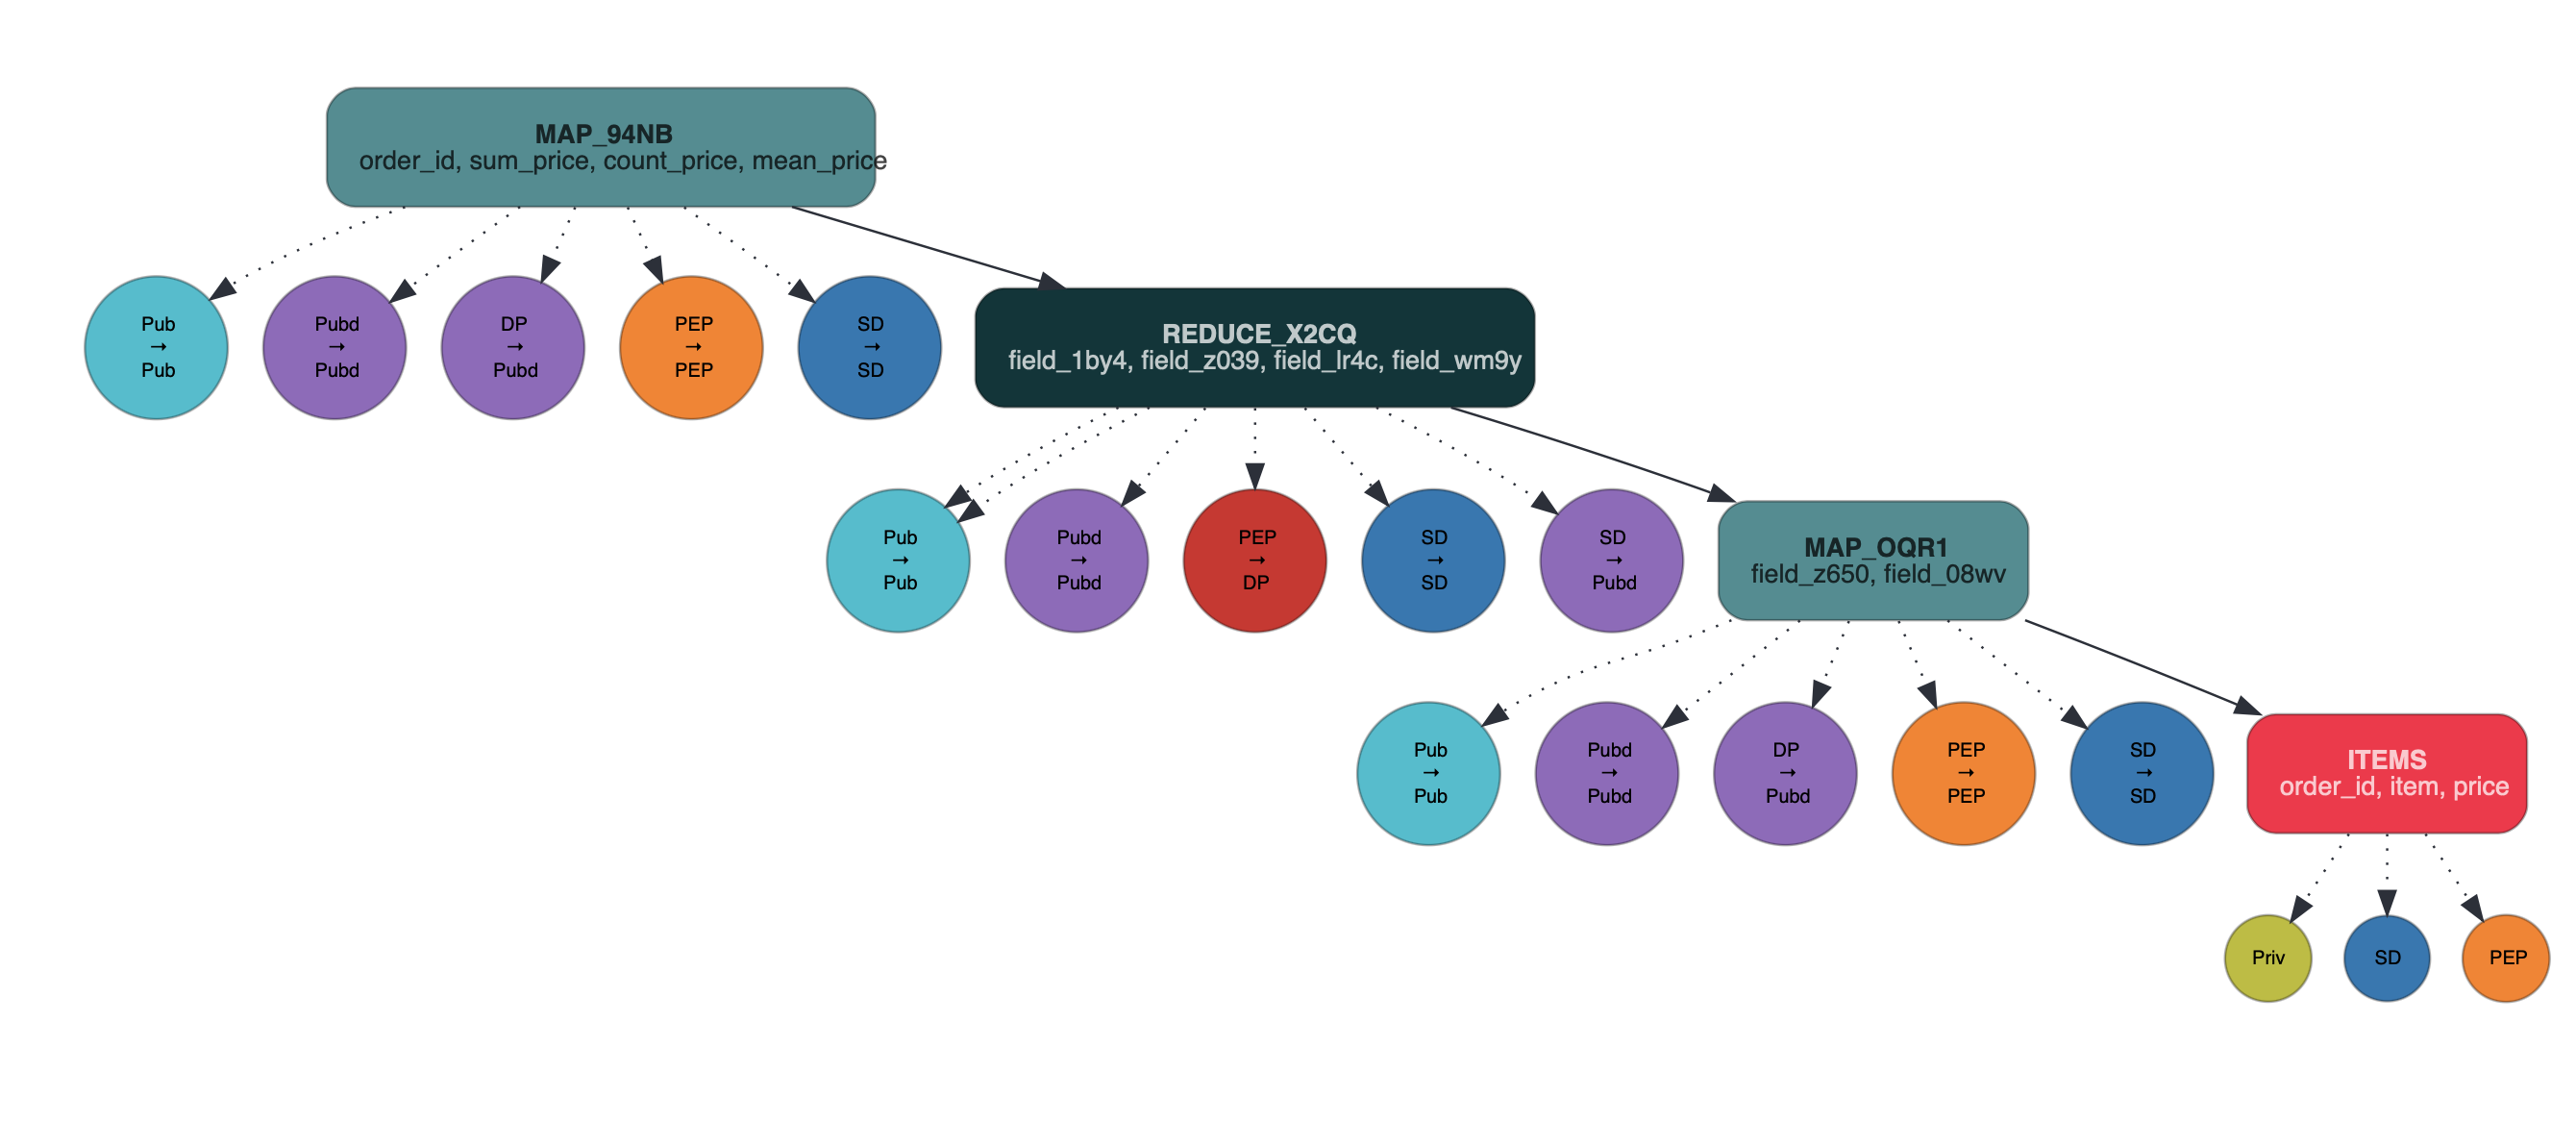
\includegraphics[width=0.75\linewidth]{rewriting_figure/rewriting_rules_setting.png}
\caption{Rule Setting: Each node in the graph (rectangle) is assigned the applicable rules (circle) for that type of node. In blue, the *→SD rules, in orange the *→PEP type rules, in purple the *→Pubd rules, and in red the *→DP rules.}
\label{fig:rule_setting}
\end{figure}

\begin{figure}[!ht]
\centering
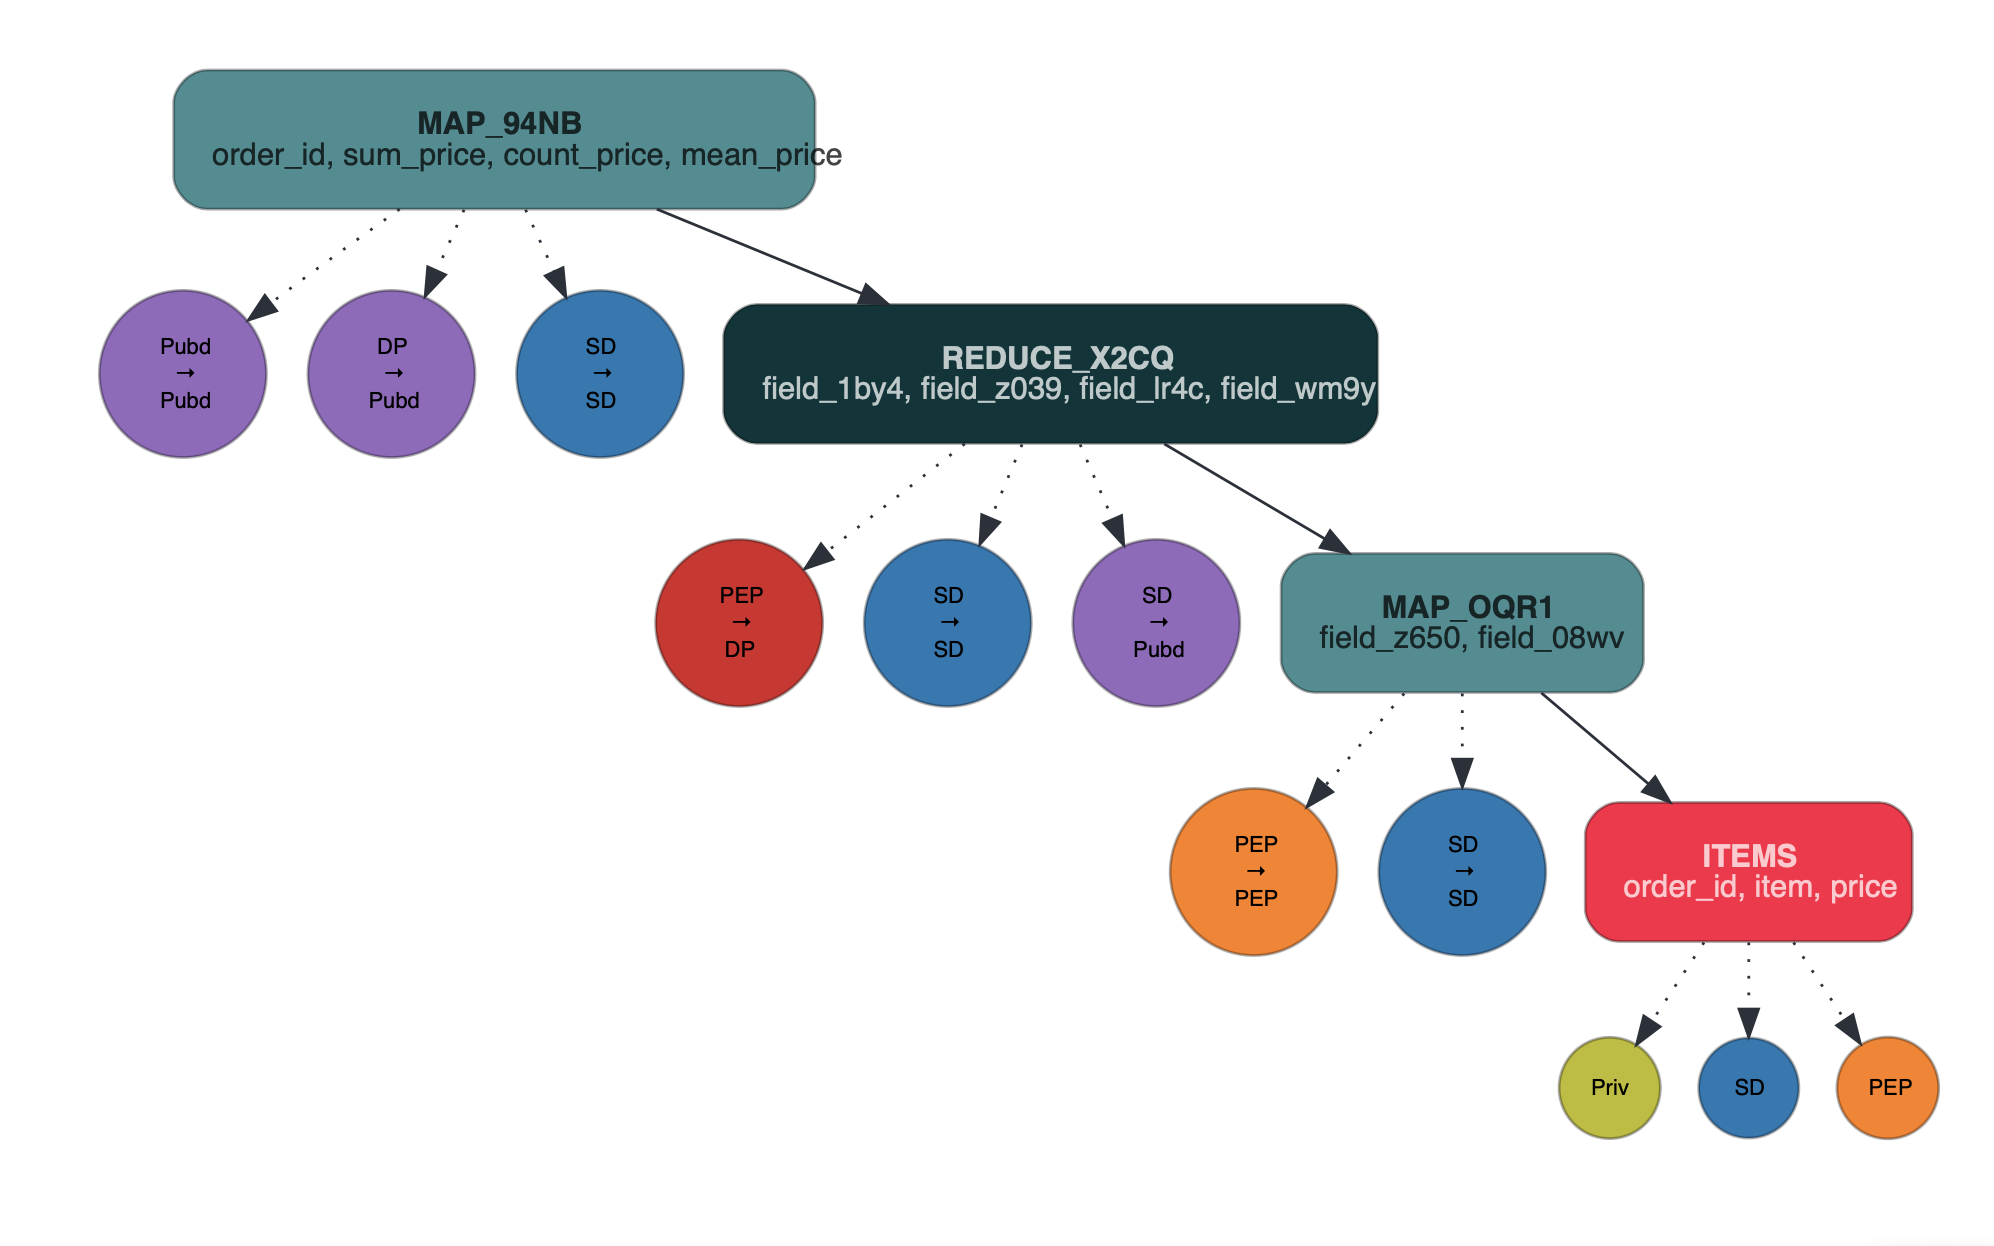
\includegraphics[width=0.75\linewidth]{rewriting_figure/feasible_rewriting_rules.png}
\caption{Rule Elimination: Only feasible rules are retained.}
\label{fig:rule_elimination}
\end{figure}


\begin{figure}[!ht]
\centering
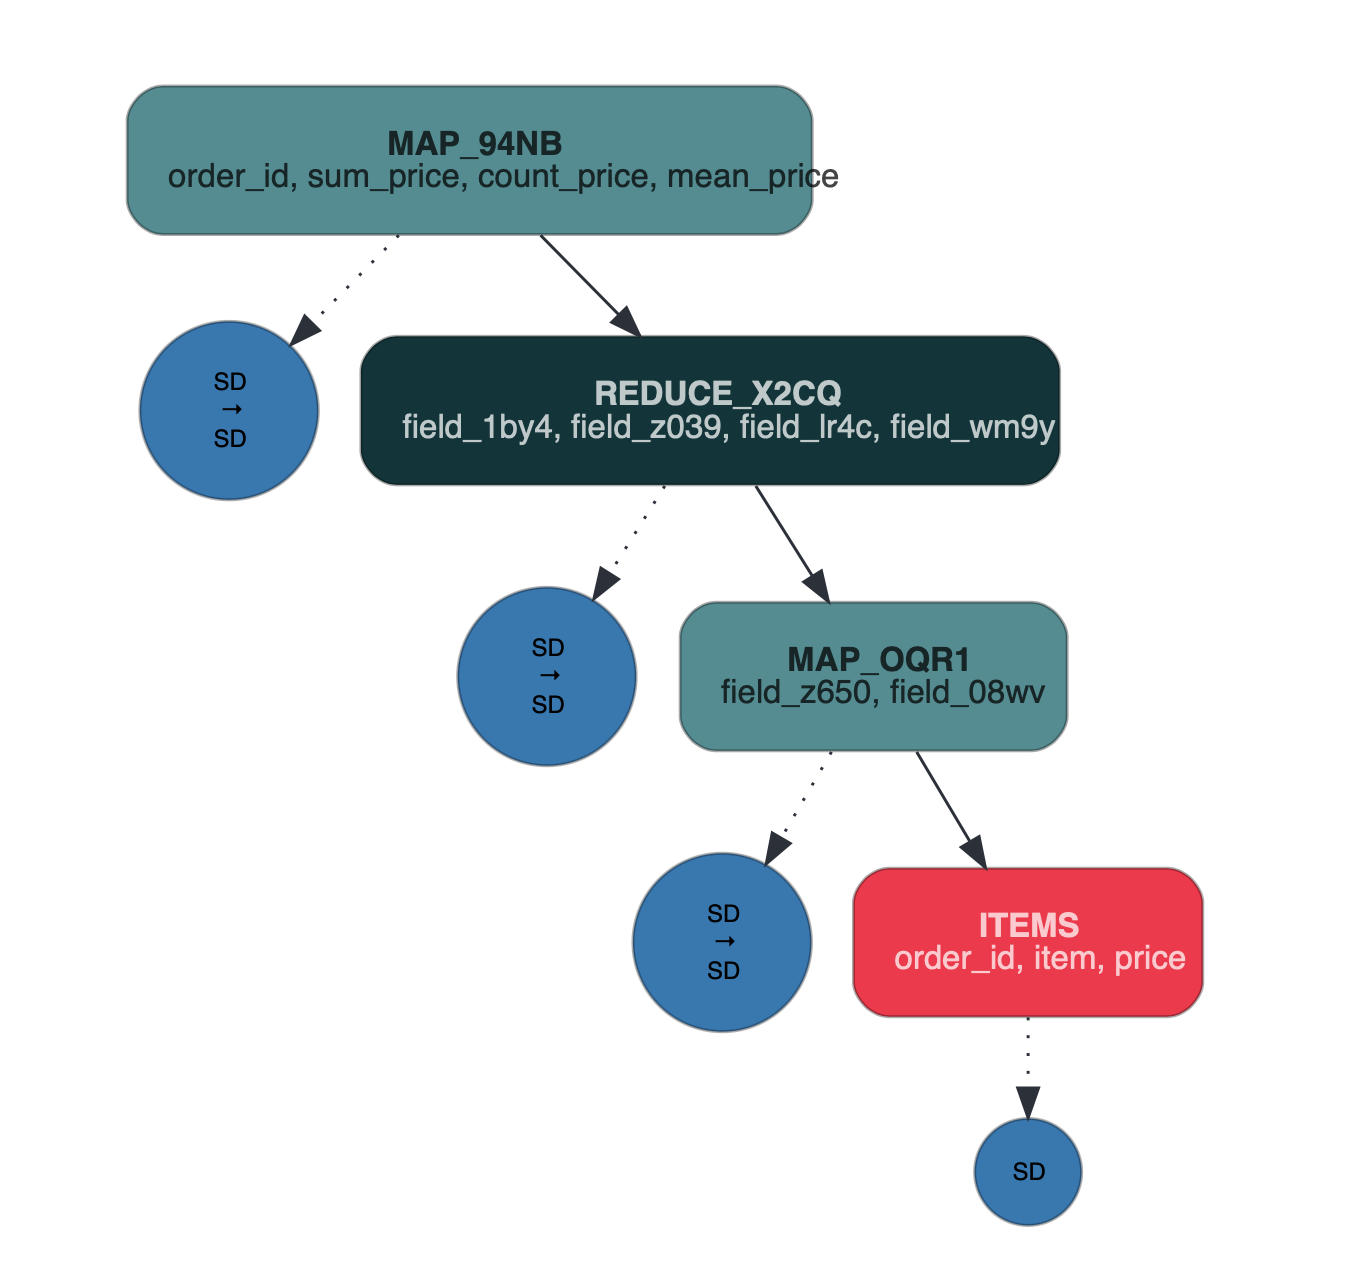
\includegraphics[width=0.75\linewidth]{rewriting_figure/sd_allocation.png}
\caption{Example of SD Allocation: The sources of the graph are substituted with their synthetic equivalent.}
\label{fig:sd_allocation}
\end{figure}


\begin{figure}[!ht]
\centering
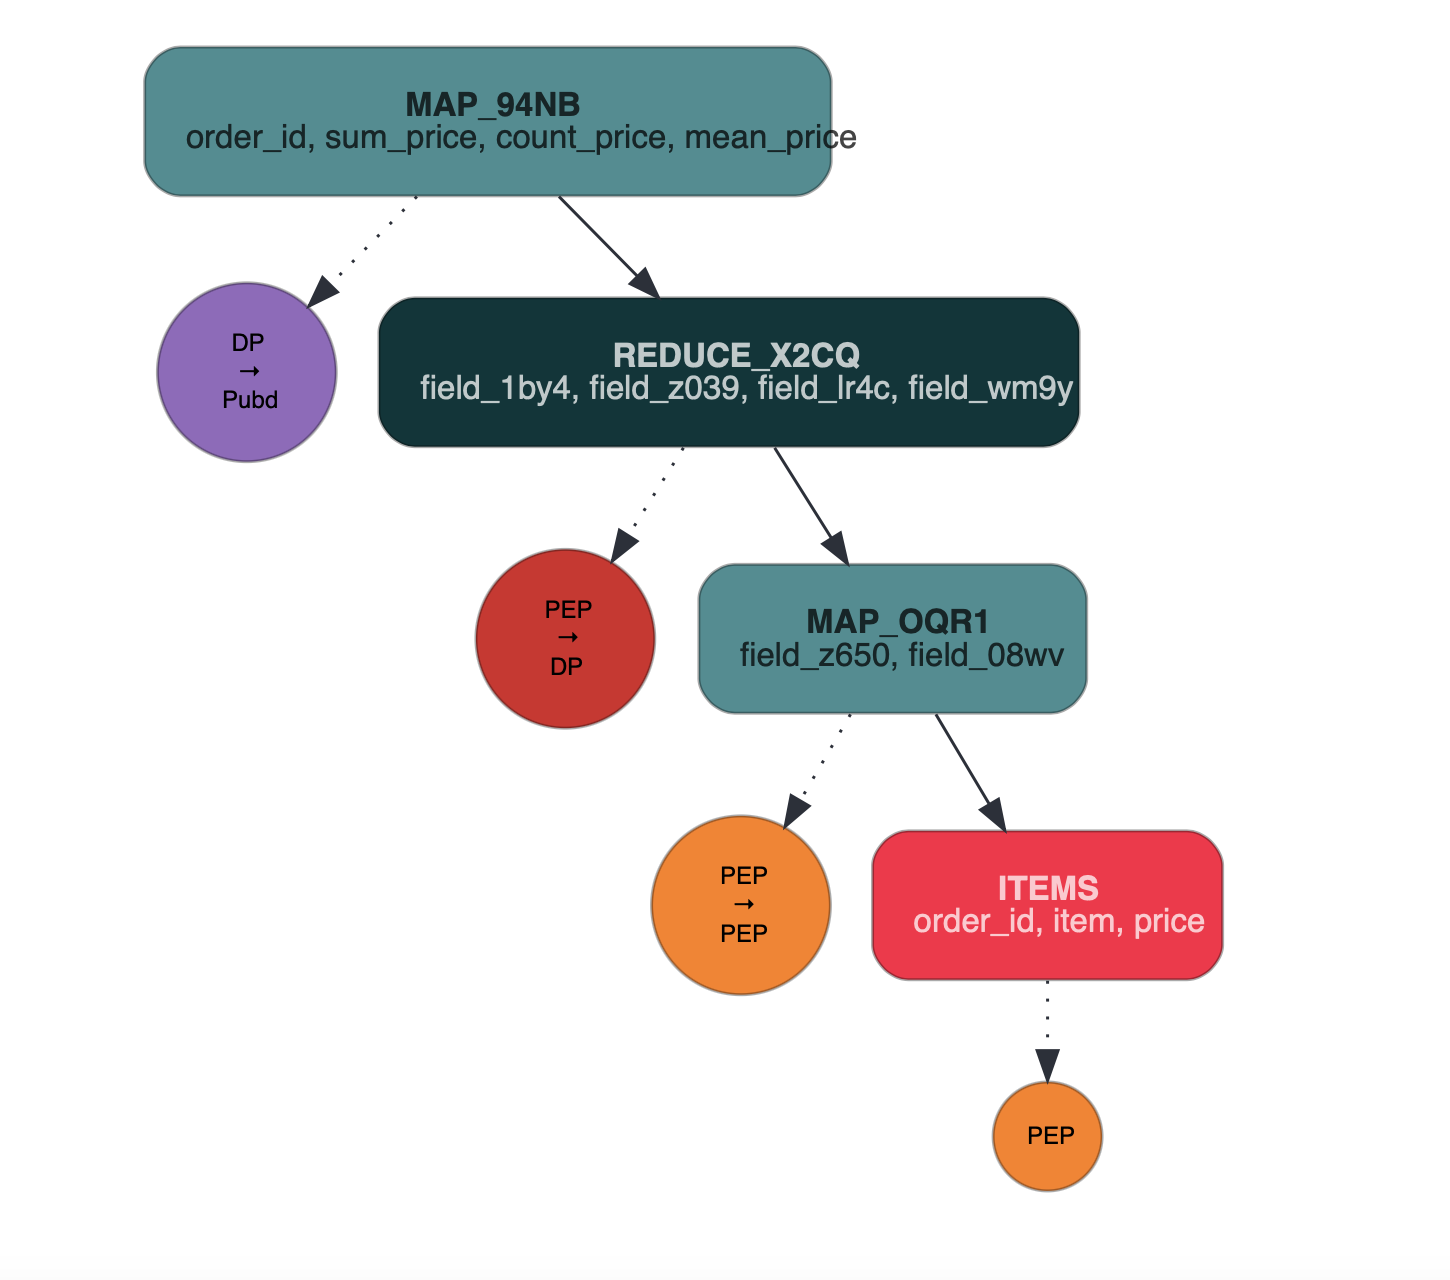
\includegraphics[width=0.75\linewidth]{rewriting_figure/dp_allocation.png}
\caption{Example of DP Allocation: Rewrite in DP as soon as necessary (and possible).}
\label{fig:dp_allocation}
\end{figure}

\end{document}
